\Chapter{Felhasznált technológiák}

\Section{C programozási nyelv}

A C programozási nyelvet Dennis Ritchi és Ken Thompson a '70-es évek elején fejlesztette ki. Általános célú programozási nyelvek közé tartozik, ami annyit tesz, hogy nem tartalmaz olyan nyelvi elemeket, amik kifejezetten egy bizonyos szakterület számára hoztak létre, ellentétben a szakterület specifikus nyelvekkel.

%\begin{figure}[h]
%	\centering
%	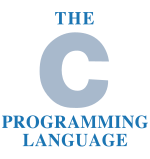
\includegraphics[scale=0.6]{images/c_prog.png}
%	\caption{C programnyelv logo.}
%\end{figure}

Kifejlesztésének elsődleges célja az volt, hogy  UNIX operációs rendszert könnyen hordozhatóvá tegyék több számítógép között.
A UNIX Assembly nyelven készült, így a hordozhatóság nagyon nehézkes volt. A szerzők először olyan magasszintű programozási nyelvet kerestek, ami alkalmas operációs rendszerek írására, emellett mégis egyszerű és hardware programozásra alkalmas. Mivel olyan nyelvet nem találtak, ami minden kritériumnak megfelelő lett volna, ezért Ritchie Thompson létrehozta a C programozási nyelvet \cite{brian1978thec}.

Ezáltal a UNIX lett az első olyan operációs rendszer, melynek jelentős része magasszintű programozási nyelven íródott.

UNIX-on kívül később számos más operációs rendszerre készítettek C fordítót, idővel piacvezető programozási nyelvek egyike lett.
Továbbfejlesztett változata a C++, ami tekinthető a C objektum orientált bővítésének.

A C nyelv legfontosabb jellemzői:
\begin{itemize}
\item \textit{Struktúrált}:
Lényege hogy minden feladat olyan kis feladatra legyen felosztva, amelyek egymással nincsenek átfedésben.
\item \textit{Szabványos}:
Minden felületen van fordítóprogramja és a fordítás egységes szabvánnyal történik.
\end{itemize}

A klasszikus \textit{"Hello World!"} C programnyelven a program neve: \texttt{pelda.c }. Ennek egy lehetséges implementációját láthatjuk a következő kódrészletben.
\begin{cpp}
#include <stdio.h>

int main(int argc, char* argv[])
{
    printf("Hello World!\n");
    return 0;
} 
\end{cpp}
Ennek a példának a fordítása például GCC fordítóval történhet az alábbi paranccsal:
\begin{cpp}
gcc -o pelda pelda.c
\end{cpp}
A programot futtatni a
\begin{cpp}
./pelda
\end{cpp}
kiadásával lehet, a kimenet pedig az alvártak szerint a
\begin{cpp}
Hello World!
\end{cpp}
lesz.

\SubSection{GCC fordító}

GCC a GNU Compiler Collection rövidítése. (A fordító logója \aref{fig:gcc}. ábrán látható.) Szabadon elérhető C fordító Linux rendszerre, de már létezik Windows-ra elkészített változata is MinGW-n keresztül. A MinGW (\textit{Minimal GNU for Windows}) egy szoftveres portja a GNU Compiler Collection-nek Windows felületre \cite{gnu2003richard}.

\begin{figure}[h]
\centering

\includegraphics[scale=0.6]{images/gcc.png}
\caption{GCC logója.}
\label{fig:gcc}
\end{figure}

\SubSection{PCRE}

A \textit{Perl Compatible Regular Expressions} rövidítve a PCRE, amely egy olyan C nyelven írt könyvtár, ami reguláris kifejezés motort valósít meg. Philip Hazel 1997-ben kezdte el kifejleszteni. Szintaxtisa erősebb és rugalmasabb mint a POSIX reguláris kifejezéseknek \cite{philip1997pcre}.

\Section{OpenGL}

Az \textit{Open Graphics Library}, rövidítve OpenGL egy részletesen kidolgozott szabvány, amit a Silicon Graphics amerikai cég fejlesztett ki az 1990-es években. Ez egy olyan programozásra alkalmas felület, amely felületen keresztül grafikus kártya kezelése és 3D programozása megvalósítható \cite{mason1999opengl}. (A könyvtár logója \aref{fig:opengl}. ábrán látható).

\begin{figure}[h]
	\centering
	
\includegraphics[scale=0.6]{images/opengl_logo.jpg}
	\caption{OpenGL logója.}
	\label{fig:opengl}
\end{figure}

\newpage

Maga a felület több ezer különböző függvényhívásból áll, melynek segítségével a programozók közvetlenül a grafikus kártya vezérlésével 3D alakzatokat rajzolhatnak ki, és ezek megvalósítását szabályozhatják közben. Felhasználása elég széleskörben zajlik, sokan használják például
\begin{itemize}
\item tervezésben, gyártásban, 
\item VR (\textit{virtuális valóság}) létrehozatalában,
\item különböző szimulátorok esetében.
\end{itemize}

Támogatott platformjai többek között a Linux és Windows, de használják még mobiltelefonokon illetve játékkonzolon.
Az első verzió 1992. június 30-án jelent meg, azóta az OpenGL-t számos alkalommal bővítették új verzió kiadásával.
Mára a legújabb verzió az OpenGL 4.6, aminek legfőbb új funkciójaként  hatékonyabb geometria feldolgozást és árnyékoló végrehajtást, illetve térbeli irányoktól függő eltolást biztosít a felhasználónak korábbi verziókhoz képest \cite{khronos1997opengl}.
